\documentclass{article}
\usepackage{tikz}
\usetikzlibrary{calc,intersections,through,backgrounds}
\begin{document}

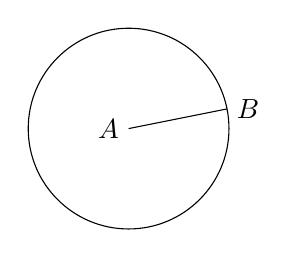
\begin{tikzpicture}

\coordinate [label=left:$A$] (A) at (0,0);
\coordinate [label=right:$B$] (B) at (1.25,0.25);
\draw (A)--(B);

\draw (A) let
	 	 \p1 = ($(B)-(A)$)
	  in
	   circle ({veclen(\x1,\y1)});
		   
	


\end{tikzpicture}

\end{document}

